%
% File acl2016.tex
%
%% Based on the style files for ACL-2015, with some improvements
%%  taken from the NAACL-2016 style
%% Based on the style files for ACL-2014, which were, in turn,
%% Based on the style files for ACL-2013, which were, in turn,
%% Based on the style files for ACL-2012, which were, in turn,
%% based on the style files for ACL-2011, which were, in turn, 
%% based on the style files for ACL-2010, which were, in turn, 
%% based on the style files for ACL-IJCNLP-2009, which were, in turn,
%% based on the style files for EACL-2009 and IJCNLP-2008...

%% Based on the style files for EACL 2006 by 
%%e.agirre@ehu.es or Sergi.Balari@uab.es
%% and that of ACL 08 by Joakim Nivre and Noah Smith

\documentclass[hidelinks, 11pt]{article}
\usepackage{acl2016}
\usepackage{times}
\usepackage{url}
\usepackage{latexsym}

% For referencing sections across the article
\usepackage{nameref}
\usepackage[]{hyperref}

% for todo notes 
\usepackage{todonotes}

% maths
\usepackage{amssymb}
% cool maths printing
\usepackage{amsmath}

\aclfinalcopy % Uncomment this line for the final submission
%\def\aclpaperid{***} %  Enter the acl Paper ID here

%\setlength\titlebox{5cm}
% You can expand the titlebox if you need extra space
% to show all the authors. Please do not make the titlebox
% smaller than 5cm (the original size); we will check this
% in the camera-ready version and ask you to change it back.

\newcommand\BibTeX{B{\sc ib}\TeX}

\title{Instructions for ACL-2016 Proceedings}

\author{Tom Byars, Cale Clark, Roman Fenlon, Charlie Lyttle, Katie McAskill, Jack Miller, Zein Said, \\
{\bf Abdullah Sayed, Laura Schauer, Jason Sweeney, Aron Szeles, Xander Wickham} \\
School of Mathematics and Computer Science, Heriot-Watt University, Edinburgh \\ {\tt {tjb10, cc164, rf104, cl157, klm12, jjm7, zs2008,}} \\ {\tt {as512, lms9, js418, as472, aw127}@hw.ac.uk}}

\date{February 2023}

\begin{document}
\maketitle
\begin{abstract}
  This should be a 6-8 page conference paper with appendices, if relevant.
  Good reports from last year: 1 and 7
\end{abstract}


\section{Introduction}
\label{sec:introduction}

\textit{from coursework spec:} main research or technical question addressed \\
Socially assistive robots (SARs) are a crucial part of the future of many sectors, for example, in education or healthcare \cite{gunson_visually_aware_2022}. Especially the latter depends on technology advancements as it is facing numerous obstacles in the future, such as increasing spendings and a growing percentage of older people. A serious lack of healthcare workers is already occurring, with 10 million more healthworkers needed worldwide by 2030 \cite{cooper_ari_2020,Health_workforce_2023}. SARs can pose a solution to the problem, as they are able to support healthcare in various ways, such as encouraging older people to keep living independently for longer or reducing caregiver burden \cite{cooper_ari_2020}.

These scenarios require SARs to be able to handle multi-party interactions as it is likely that more than one person will interact with the system. Compared to handling dyadic interactions, handling multi-party conversations includes more complex challenges, such as Speaker Recognition, Addressee Recognition, Response Selection (summarised in “who says what to whom“) and turn-taking \cite{Group_1_unpublished_paper,Johansson_Skantze_2015}.

\textit{Include here what exactly we examined about turn-taking}

In this work, we propose a model trained on multi-party human-human conversation data. We collected the data from recordings of special “Who wants to be millionaire?“ episodes where two candidates collaborated to answer the host's questions.

\textit{Include results here.}


\section{Background}
\label{sec:background}

\textit{from coursework spec:} literature review / related work, including a critical analysis of the field, and commentary on applicability of the technologies and methods used in emerging technologies and application areas

\subsection{Socially Assistive Robots}
\label{subsec:socially_assistive_robots}
For healthcare, as well as for any other sector, the difficulty of successfully designing SARs lies in creating robots that can effectively converse with humans and adhere to social norms \cite{moujahid_multi_party_2022}. The more expressive a robot is, the more it will be perceived as intelligent, conscious and polite \cite{moujahid_multi_party_2022}. To achieve such a positive perception, multiple parts need to be combined into one conversational system, such as the ability to carry out visually grounded as well as task-based dialogues, to perceive and discuss its environment and to chit-chat \cite{gunson_visually_aware_2022}.

The SPRING project conducts research on a SAR robot that is deployed in an eldercare hospital reception area \cite{addlesee_comprehensive_2020}. The conversational system is deployed on humanoid ARI robot produced by Pal Robotics \cite{palrobot}. ARIs capabilities can be extended with custom AI algorithms, in the case of SPRING-ARI a visual perception system, a dialogue system, and a social interaction planner \cite{addlesee_comprehensive_2020}. While the SPRING-ARI system successfully demonstrates that task-based, social and visually grounded dialogue can be combined with physical actions, it still lacks the ability to handle conversations with more than one person simultaneously \cite{addlesee_comprehensive_2020}.

\subsection{Multi-party Human Robot Interaction}
\label{subsec:multi_party}
As stated above, the endeavour to create conversational systems becomes considerably more difficult when dealing with multi-party interactions \cite{Group_1_unpublished_paper}. Especially turn-taking poses a central problem. It is defined as follows:

\begin{quote}
  The rules of turn-taking organize the conversation into turns, during which one of the participants has the right to speak while the others agree to listen \cite{Żarkowski_2019}
\end{quote}

In dyadic conversations, there are only two roles a participant can take: speaker or listener, hence it is clear when and to whom the turn is yielded. In multi-party conversations, participants can take multiple roles, therefore turn-taking needs to be coordinated \cite{Johansson_Skantze_2015}. Humans signal their intents mostly through gaze, but also through pauses, prosody, and body positioning \cite{Żarkowski_2019}. To copy this behaviour, earlier models for conversational systems relied on silence time-outs to coordinate turn-taking, however, this approach is found to be too simplistic \cite{skantze_turn_taking_2021}. Instead, mimicking human turn-taking behaviour better by using a combination of verbal and non-verbal cues leads to robots that are better perceived \cite{moujahid_multi_party_2022}.

\textit{State exactly the gap that we will fill - whatever that will be}


\section{Data Collection}
\label{sec:data_collection}

\begin{itemize}
  \item (Laura) Talk about multi-party data collection
  \item (Aron and Katie) How we collected our data, describe the intents we used to label the data
  \item (Aron and Katie) Cohen's Kappa for our data collection method: probably need to annotate a couple of transcripts twice for reporting on this
\end{itemize}

Data collection was performed in-house, by the team. We first collected all available recordings of Who Wants to Be a Millionaire with two participants. Using the YouTube API, we managed to get the transcripts for the vast majority of recordings. To annotate these transcripts, we came up with the following unified set of annotations that would allow us to capture as much information as possible, without saturating the data.
\begin{itemize}
  \item question - The system presents the question
  \item options - The system presents the options
  \item chit-chat - Speech not related to the quiz
  \item offer-answer() - A player presents an answer to the other player
  \item offer-to-answer - A  player signals that he/she knows the answer
  \item check-answer - A player checking if the other player knows the answer
  \item agreement - Agreement between players about the answer
  \item ask-agreement - A player asks the other player for confirmation about their answer
  \item accept-answer System considers answer the final answer
  \item final-answer() - Players give final answer
  \item confirm-agreement - System tries to confirm the final answer with participants
  \item confirm-final-answer - Participants confirm their answer is final
\end{itemize}

\subsection{Cohen's Kappa Coefficient}
As the system uses the annotations to train the system, ensuring that they are reliable and consistent is essential for accurate training. Cohen's kappa was used on a sample of the completed transcripts to evaluate their accuracy. Cohen's kappa measures the reliability between raters on categorical data. It is said to be more accurate than calculating the agreement as it accounts for agreements happening by chance. \todo{add source}

To calculate Cohen's kappa, a sample of four transcripts were re-annotated by a team member, without them seeing the original annotations to remove any possible bias. This amounts to approximately 15\% of the total transcripts.

Every occurrence by both raters of each annotation label was gathered. An overall agreement rate was calculated using -

\begin{equation} \label{eq:kappa}
  \begin{split}
    Agreement & = \frac{total \: Agreed}{total} \\
    % Agreement & = \frac{329}{341} \\
    Agreement & = 0.9684
  \end{split}
\end{equation}

This alone is not reliable enough to trust.\todo{source} To calculate the chance of an agreement happening between the two raters, first the probability of a rater choosing a label was calculated. This was done for each rater for every label using -

\begin{equation}
  Prob(R_x[label]) = \frac{R_x \: Total \: for \: [label]}{total}
\end{equation}

Then the chance of agreement for each annotation label was calculated using -

\begin{equation}
  \begin{split}
    &ChanceAgreement[label] = \\
    &Prob(R_1[label]) * Prob(R_2[label])
  \end{split}
\end{equation}

The overall chance of agreement was calculated by summing the chance of agreements for each annotation label.

Finally, the kappa score was calculated.

\begin{equation}
  \begin{split}
    KappaScore & = \frac{Agree - ChanceAgree}{1 - ChanceAgree} \\
    KappaScore & = 0.9601
  \end{split}
\end{equation}

According to Cohen \todo{add source}, a Kappa score of 0.9601 is interpreted as almost perfect agreement. From this, the annotation of transcripts can be concluded as reliable and therefore the training model will accurately learn from this data.

\section{Design and Implementation}
\label{sec:implementation}

\begin{itemize}
  \item \textit{from coursework spec:} design and implementation of the system: components and architecture
  \item Jack's System Graph
\end{itemize}

\subsection{Automatic Speech Recognition}
\label{subsec:asr}

To enable interaction between users and the conversational system, the first step is to transform user's speech into text, in order to pass text further onto intent recognition (NLU). Transforming audio into text works through Speech-To-Text (STT)software. In recent years, STT systems are becoming more accurate and fast, however, research found that none of the existing systems can yet reliably handle conversations in real time \cite{Addlesee_Yu_Eshghi_2020}.

The system we \todo{Get rid of pronoun} have built required two things specifically from the ASR that are not available in all ASR systems. The first being real time transcription. As our system is going to be used on a robot, it must transcribe what the user is saying in real-time to avoid long delays before the system responds. For a usable system in this context the time taken for a system to respond can be no longer than the delay a human would leave before responding or only marginally longer. In addition, our system requires diarization. Diarization is the process of taking a single audio file, in which two or more people are speaking, and determining who is speaking at what time. As two users would be speaking to each other and to our system, our system must recognise when each individual is talking. \todo{Those two sentences have the same content} This would allow us to track the intents of each user and determine when they have agreed with each other.
We tried many of the most popular STT systems including Amazon's Transcribe, IBM's Watson and locally running Pyannote. These are all valid options for transcription but lack real-time diarization, that is, diarising the speech as it is spoken.
Finally, we \todo{Get rid of pronoun} settled with Google's Cloud Speech-to-Text API due to its high accuracy, real-time transcription capabilities, and customisability. Also, as it is widely used, resources available for troubleshooting and integration were readily available.

As well as these reasons, Google's API boasted diarization capabilities, along with its real-time transcription capabilities seemed to fit our use case. However, in use, diarization was inaccurate and often grouped two separate speakers together or split sentences up seemingly at random. This became even more apparent when two users were speaking over each other. This is in accordance with the findings of \cite{addlesee_comprehensive_2020}. Diarization is quite resource-heavy meaning that running a diarization algorithm in real time takes an extreme amount of resources and, unfortunately, is not feasible on normal, consumer-grade hardware. And although diarization APIs exist, they do not respond fast enough for our use case. This made Google's diarization unusable for our system, therefore we decided to handle the diarization separately and integrate it with the real time Google transcription.

\subsection{Natural Language Understanding}
\label{subsec:nlu}

\begin{itemize}
  \item Short description of RASA
  \item Explain the aim (detecting intents)
  \item Refer to the intents described in \ref{sec:data_collection} \nameref{sec:data_collection}
  \item Evaluation - show different versions of the model: difference in F-Score, Confusion Matrix, ...
\end{itemize}

\begin{figure}
  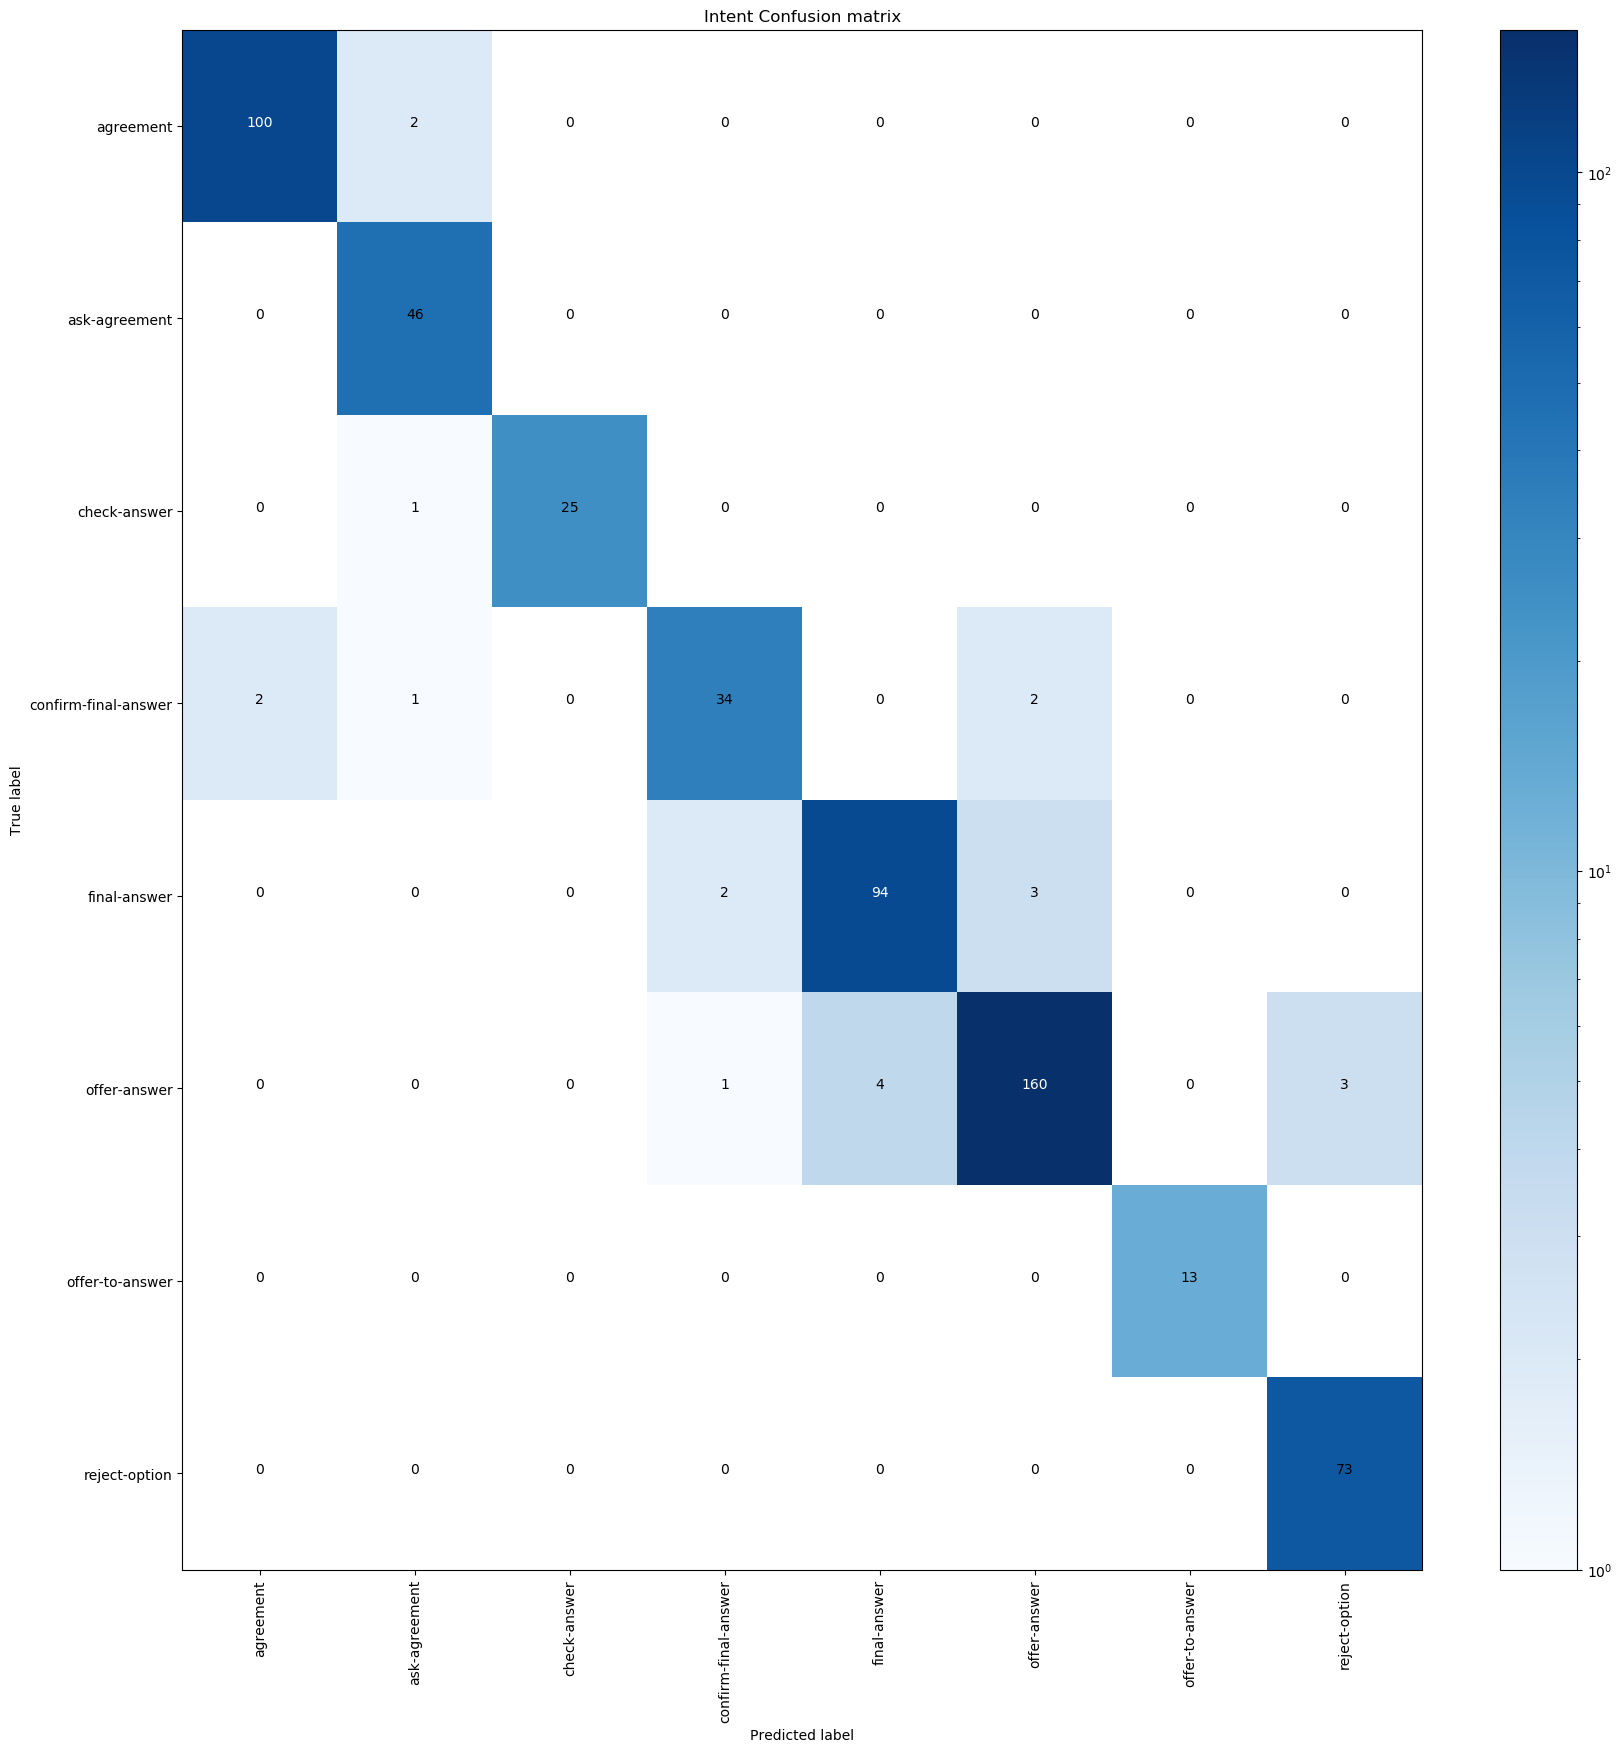
\includegraphics[width=\columnwidth]{../Rasa/Evaluation/Clean_Model/intent_confusion_matrix.png}
  \caption{Intent Recognition Confusion Matrix}
  \label{fig:intent_confusion_matrix}
\end{figure}

\subsection{Dialogue Management}
\label{subsec:dialogue_management}

\begin{itemize}
  \item Clearly explain 2 parts (State-Machine and NN)
  \item State-Machine: high-level control, handles things we have no data for, eg. pauses
  \item NN: Report on differences between RNN and LSTM and why the choice for the LSTM has been made
  \item (optional): Comparison to RASA rule-policy
\end{itemize}

\subsection{Natural Language Generation}
\label{subsec:nlg}

To make the system feel more unique and less robotic, we made use of Natural Language Generation (NLG) for the phrases that the “host” says to the participants. We used OpenAI's API, specifically “gpt-3.5-turbo”, the same version that is used in ChatGPT. This allowed us to prompt for different outputs for the system that convey the same information. For example, when receiving a correct answer, “Yes, that's it! Well done!” and “You got it! Great job!” are both possible outputs. There are 50 different options for each response the “host” can say.


\section{Evaluation}
\label{sec:evaluation}

\textit{from coursework spec:} evaluation of the system and presentation of the results

\subsection{Methodology}
\label{subsec:methodology}
In this study, we performed extrinsic and intrinsic evaluations. The extrinsic evaluation focused on both subjective and objective measures of the system's performance. The subjective measures included the user's enjoyment and perception of the system's natural behaviour, while the objective measures included the number of turns taken and the agreement rate. Additionally, the correlation between correct answers and enjoyment was also examined. Overall, the evaluation aimed to assess the effectiveness of the system in engaging users and providing accurate responses.

The evaluation focused on intrinsic measures of individual components in a multi-party conversational system. The components were assessed separately, with ASR being evaluated using the word error rate, NLU using precision, recall, accuracy, and F1 score, DM IDK YET, and NLG using n-gram-based overlap with BLEU. The aim was to assess the performance of each component and identify areas of improvement.

Additionally, the evaluation also aimed to test the hypothesis that using verbal cues instead of silence cues in a multi-party conversational system increases user interaction and satisfaction with the system. This hypothesis needed to be statistically proved or disproved through significance testing.
\subsection{Experiment Layout}
\label{subsec:experiment_layout}
The experiment followed a between-subjects design. Every participant was required to read and sign a consent form before they can play the quiz. This was an in-person experiment, with the quiz running on a laptop, where participants can see the questions and the options. Members of the experiment were required to play the quiz at least once. However, they were encouraged to play as many times as they can. After they no longer wished to play, they were asked to complete a questionnaire about their experience. The questionnaire queried them on their experience using a five-point Likert scale.

\subsection{Results}
\label{subsec:results}

\begin{itemize}
  \item ASR results
  \item NLU result
  \item DM result
        NLG result
  \item questionnaire result
\end{itemize}

\section{Conclusion}
\label{sec:conclusion}

\subsection{Ethical Reflection}
\label{subsec:ethics}

\section{Future Work}
\label{sec:future_work}

\textit{from coursework spec:} suggestions for future work

To further improve on NLG within this system, some content moderation could be performed on the generations, to ensure that there are no inappropriate outputs, this can be done entirely within OpenAI's API.  Also, the system could be updated to make use of GPT-4, which at this current time is not publicly available.



\section*{Acknowledgments}
\label{sec:acknowledgments}

The acknowledgments should go immediately before the references.  Do
not number the acknowledgments section. Do not include this section
when submitting your paper for review.

% include your own bib file like this:
%\bibliographystyle{acl}
%\bibliography{acl2016}
\bibliography{references}
\bibliographystyle{acl2016}

\appendix

\section{Supplemental Material, Appendix}
\label{sec:supplemental}


\end{document}
